\section{Méthodologie}~\label{sec:metho}
Afin de valider l'hypothèse que les modèles de force de contact linéaires sont adéquats pour les~\ac{VSS}, un modèle dynamique planaire est détaillé dans la~\autoref{sec:modele}.
Un protocole expérimental permettant d'obtenir les données nécessaires à l'évaluation des forces a été mis en place et exécuté.
Ce protocole est présenté dans la~\autoref{sec:protocole}.

\subsection{Théorie}~\label{sec:modele}
Afin d'évaluer l'exactitude des modèles de forces de contact linéaires, nous avons développé un modèle dynamique planaire de \ac{VSS}, qui est montré dans la~\autoref{fig:modele}.
Un repère global ainsi qu'un repère du corps du robot sont définis.
La totalité des quantités définies dans cette section sont exprimées dans le repère du corps du robot.
La vitesse de rotation des roues de gauche $\omega_l$ sont identiques, il en est de même pour la vitesse de rotation des roues de droite $\omega_r$. 
Il est important de noter que bien que le modèle illustré sur la~\autoref{fig:modele} ne comporte que deux roues par côté, ce modèle fonctionne pour tout \ac{VSS} comportant deux roues ou plus sur chaque côté.
La vitesse du corps du véhicule $\bm v = [v_x, v_y]^T$ comporte une composante longitudinale et une composante latérale.
Le corps du robot a également une vitesse angulaire $\omega$.

\begin{figure}[htpb]
	\centering
	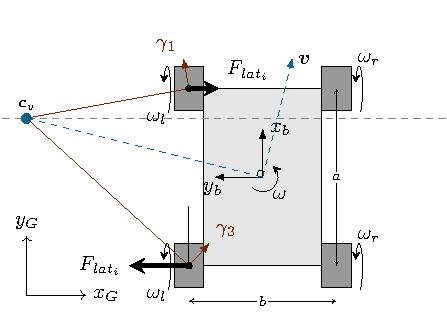
\includegraphics[width=0.48\textwidth]{figs/modele.pdf}
	\caption{Modèle dynamique planaire d'un \ac{VSS}.
			Le vecteur de vitesse du corps du robot ainsi que le centre de rotation instantané sont illustrés en bleu.
			Un angle de glissement est illustré en rouge.
			Dans ce modèle, seules les forces latérales subies par les roues sont considérées.}
	\label{fig:modele}
\end{figure}

En fonction de la vitesse du corps du robot, il est possible de définir la position d'un centre de rotation instantané $\bm c_v$.
La position de ce centre de centre de rotation instantané est calculée comme dans~\citep{Mandow2007} :
\begin{equation}
	\bm c_v = \begin{bmatrix}
	x_{c_v} \\ 
	y_{c_v} \\
	\end{bmatrix} = \begin{bmatrix}
	\frac{v_y}{\omega} \\ 
	\frac{v_x}{\omega} \\
	\end{bmatrix} \text{,}
	\label{eqn:icr}
\end{equation}
où $x_{c_v}$ et $y_{c_v}$ sont les positions longitudinale et latérale du centre de rotation instantané dans le repère du corps du véhicule.

Afin de simplifier le modèle, seules les forces latérales subies par le véhicule sont prises en compte.
Ces forces ont une orientation contraire à l'angle de dérive de chaque roue $\gamma_i$, qui peut être calculé ainsi, comme dans~\citep{Maclaurin2011} :
\begin{equation}
\begin{cases}
	\gamma_i = \arctan(\frac{a_i - x_{c_v}}{y_{c_v} - b_i}), & \text{if } b_i y_{c_v} > 0 \text{ et } b_i > y_{c_v} \\
	\gamma_i = \arctan(\frac{a_i - x_{c_v}}{b_i - y_{c_v}}) & \text{autrement} \text{,}
\end{cases}
\label{eqn:angles}
\end{equation}
où $a_i$ et $b_i$ sont les positions longitudinales et latérales du point de contact de la roue $i$ dans le repère du véhicule.

Ces positions sont positives ou négatives dépendant de la roue en question.
La condition est introduite afin de prendre en compte le cas où le centre de rotation instantané est situé entre les roues du véhicules.
Dans ce cas, l'angle de dérive des roues internes doit être calculé autrement.
Les forces de contact latérales subies par chaque roue $F_{lat_i}$ peuvent ensuite être calculé selon le modèle linéaire :
\begin{equation}
	F_{lat_i} = -\alpha_{lat} \gamma_i \text{,}
	\label{eqn:forces}
\end{equation}
où $\alpha_{lat}$ est un coefficient de friction lié à la nature du sol sur lequel le robot opère.
Comme les forces latérales sont des forces de friction, celles-ci sont de sens opposé à la direction du mouvement donc à l'angle de dérive. 
Alternativement, les forces latérales peuvent être calculé en substituant l'angle de dérive par la vitesse latérale du point de contact $v_{c_i}$ de chaque roue dans l'\autoref{eqn:forces}~\citep{Seegmiller2016}.
De cette manière, il est possible d'exprimer le système d'équations du mouvement dans la direction latérale du robot :
\begin{equation}
	\sum_{i=1}^{n} F_{lat_i} = m a_{lat} \text{,}
	\label{eqn:forces_sum}
\end{equation}
où $m$ est la masse du véhicule, $a_{lat}$ est son accélération latérale et $n$ est son nombre de roues total.

Pour ce modèle, nous considérons que le véhicule opère en régime permanent, ce qui implique que les accélérations longitudinale et angulaire sont nulles.
Pour ce qui est de l'accélération latérale, celle-ci est équivalent à l'accélération centripète ou d'Alembert, que l'on calcule comme~\citep{Maclaurin2011} :
\begin{equation}
	a_{lat} = m \frac{v^2}{R_c} = \frac{v^2}{\sqrt{x_{c_v}^2 + y_{c_v}^2}} \text{,}
	\label{eqn:centripete}
\end{equation}
où $R_c$ est le rayon de courbure du véhicule. 

Dans le cas où le modèle de force de contact linéaire présenté dans l'\autoref{eqn:forces} est exact, l'égalité présentée à l'\autoref{eqn:forces_sum} doit être respectée.
Il est certain qu'en raison des incertitudes liées à l'opération d'un véhicule et au bruit de capteurs, celle-ci ne sera pas respectée mais ce rapport vise à quantifier l'erreur liée à ce genre de modèle pour les \ac{VSS}.

\subsection{Protocole expérimental}~\label{sec:protocole}
Afin d'évaluer l'égalité l'exactitude du modèle présenté dans la~\autoref{sec:modele}, nous avons enregistré des données de conduite avec un \ac{VSS}. 
Un Warthog de la compagnie \textit{Clearpath Robotics} a été utilisé, une photo de cette plateforme est montrée sur la figure~\autoref{fig:warthog}.
Cette plateforme est un \ac{VSS} à 4 roues et ayant une masse $m$ de \SI{260}{\kg}.
Afin de valider notre hypothèse pour plusieurs vitesses angulaires, nous avons défini 10 vitesses angulaires commandées distintes pour l'expérience.
Ces vitesses commandées sont définies dans le vecteur $\omega_c = [0.0, 0.1, 0.2, 0.4, 0.75 ,1.25, 2.0, 3.0, 4.0, 5.0]$.
La sélection de ces vitesses a été faite dans le but d'évaluer une plus grande quantité de vitesses angulaires faibles et tenter d'observer le point de saturation des pneus.
Afin d'éviter les phénomènes liés à la déformation du terrain pour les vitesses angulaires élevées, nous avons classé les éléments de $\omega_c$ de manière aléatoire.
Pour ce qui est de la vitesse longitudinale commandée, celle-ci a été fixée à \SI{0.5}{\m\per\second} afin de limiter la durée de l'expérience.
Pour respecter l'hypothèse de régime permanent, chaque commande a été exécutée par le robot pour une durée de \SI{10}{\second}.

\begin{figure}[htpb]
	\centering
	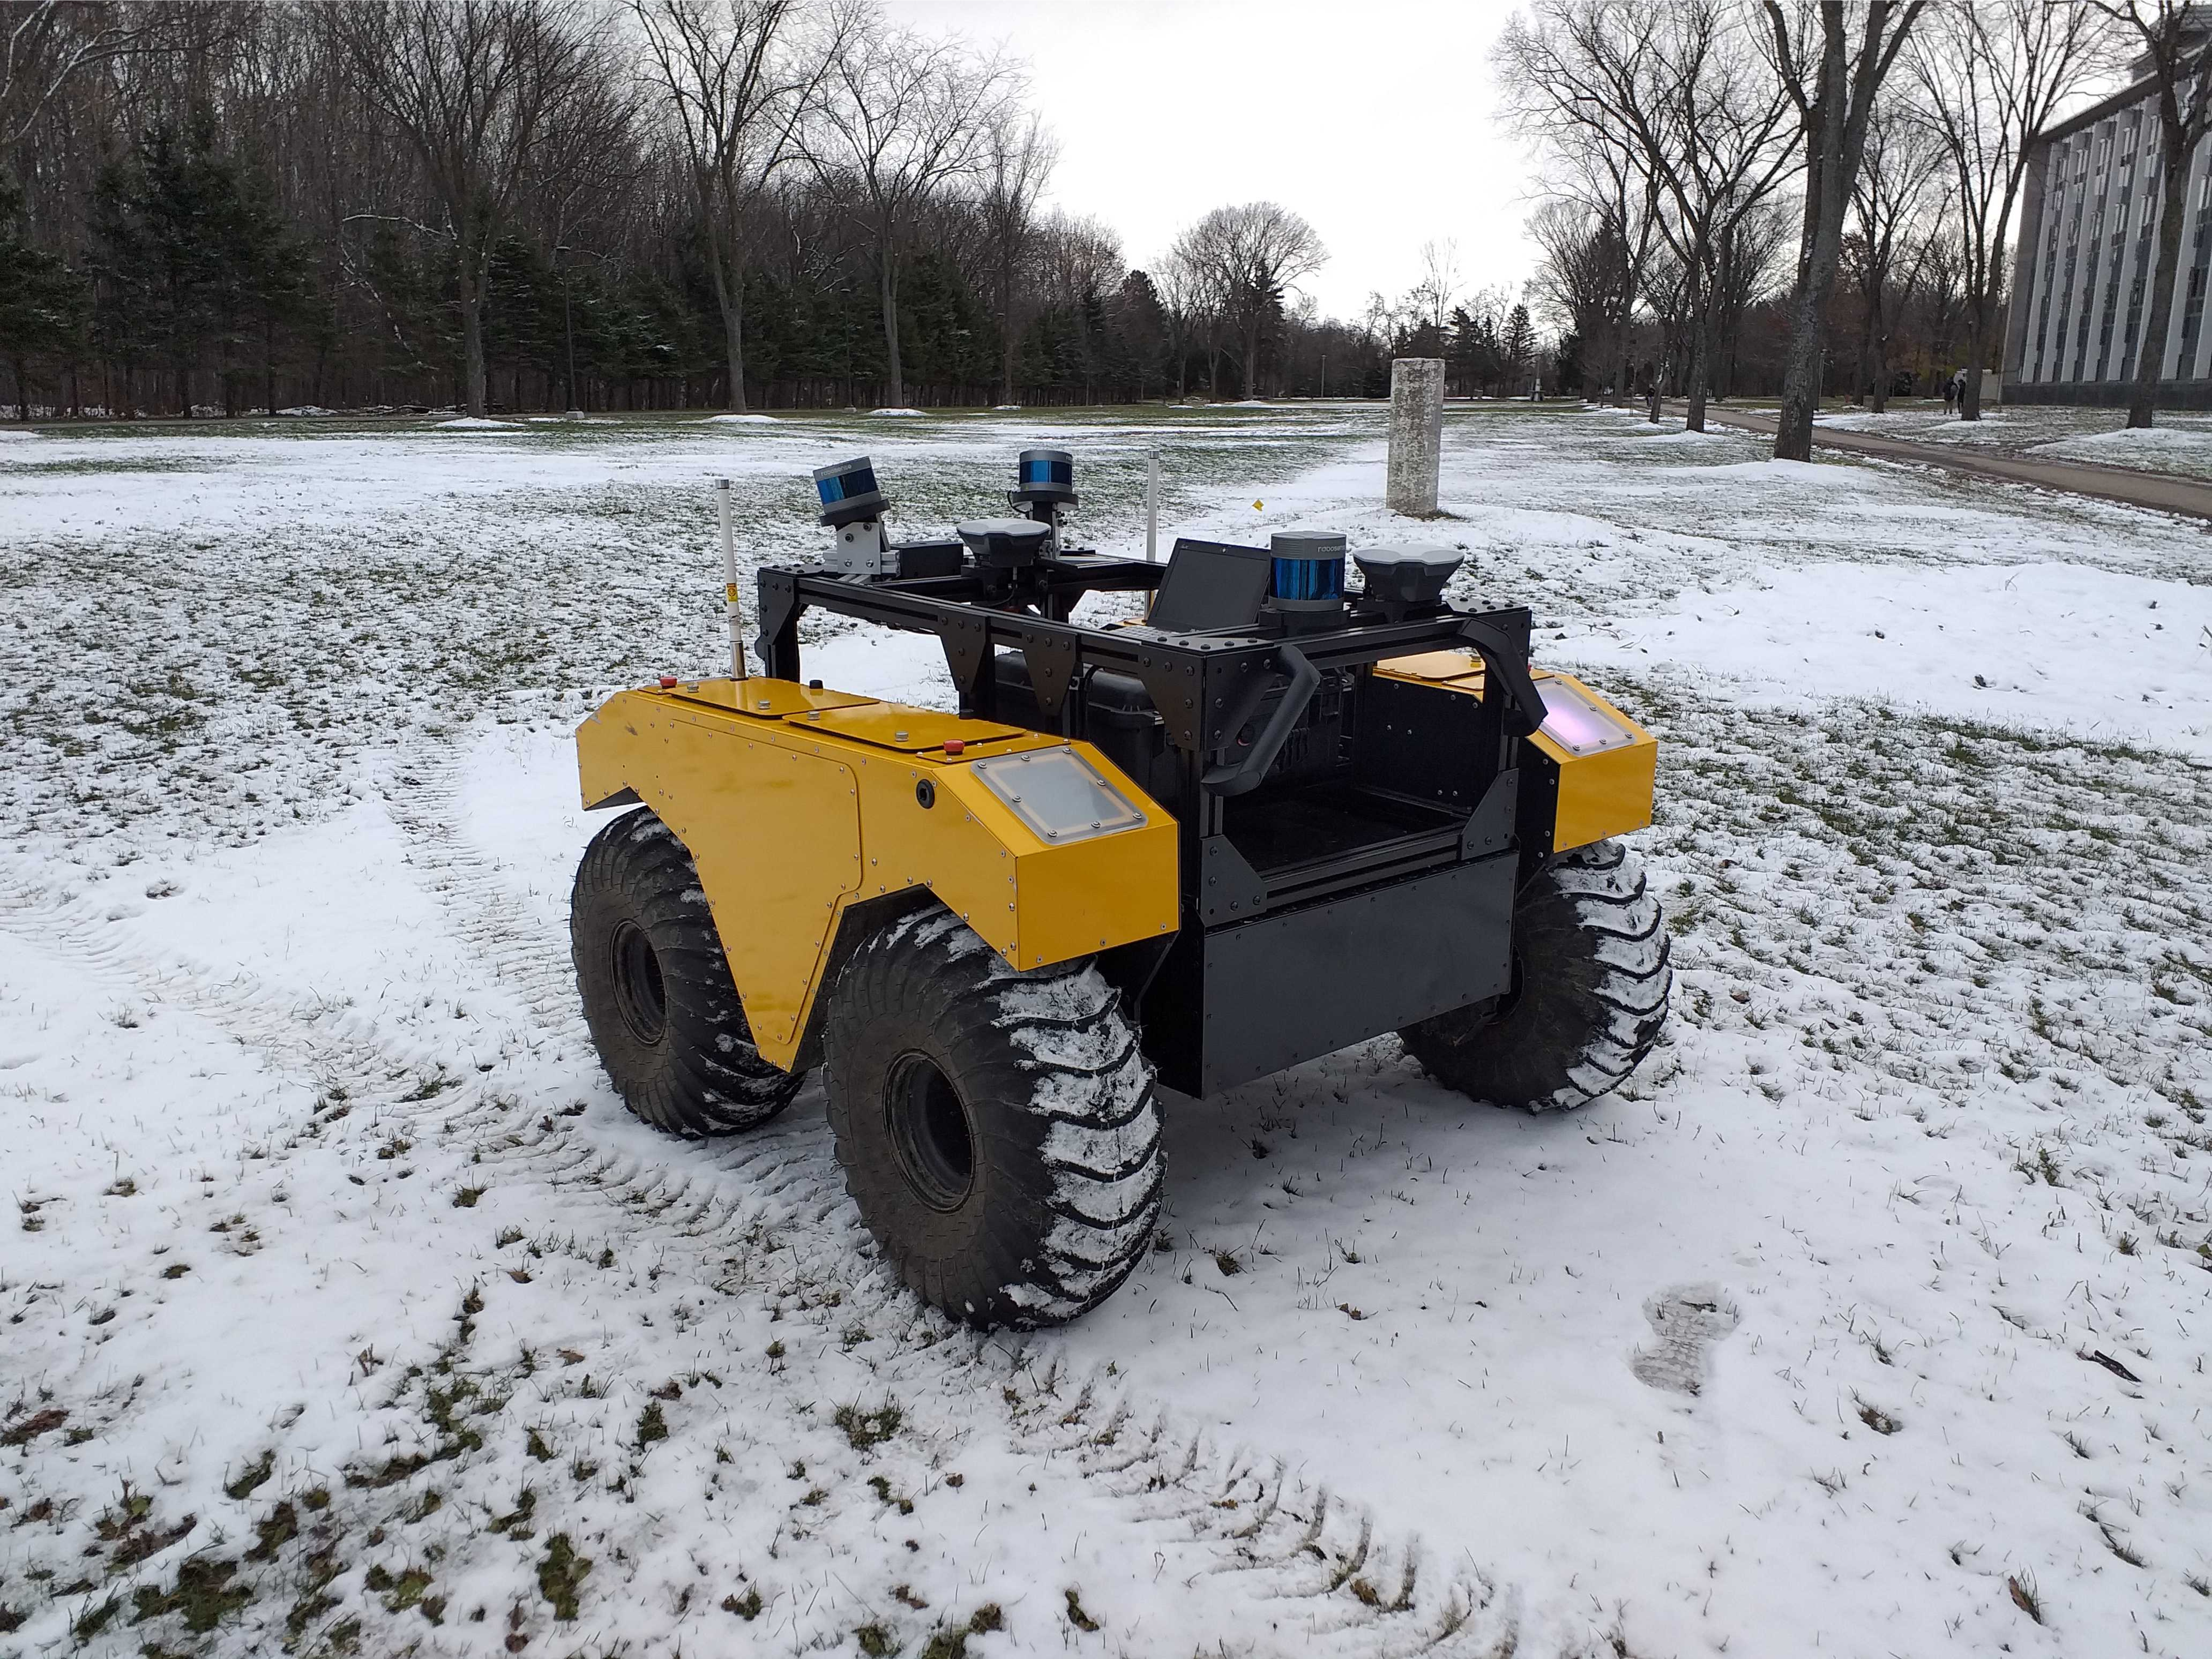
\includegraphics[width=0.4\textwidth]{figs/warthog.pdf}
	\caption{Photo du Warthog utilisé pour la phase expérimentale de ce projet.
		Cette plateforme est équipée d'un lidar Robosense RS-32 et d'une centrale inertielle Xsens MTi-10 pour se localiser.
		Le véhicule a été conduit sur le grand axe du campus de l'Université Laval, à Québec au mois de Novembre.}
	\label{fig:warthog}
\end{figure}

La plateforme comporte des encodeurs aux roues qui permettent de mesurer leur vitesse angulaire.
Une centrale inertielle permet quand à elle de mesurer la vitesse angulaire du corps du véhicule.
L'estimation de la position du corps du véhicule est réalisée en recallant des nuages de points grâce à l'algorithme \ac{ICP}~\citep{Pomerleau2015}.
La librairie \texttt{libpointmatcher}\footnote{\url{https://github.com/ethz-asl/libpointmatcher}} a été utilisée pour implémenter cet algorithme dans le cadre ce cette expérience.
Toutes les données sont enregistrées et exportées grâce au logiciel de gestion de flux de données Robot Operating System (ROS)\footnote{\url{https://www.ros.org/}}.
Le traitement des données a été réalisé grâce au langage de programmation \texttt{Python} et le code est disponible en ligne\footnote{\url{https://github.com/DomBaril/GSO-7107}}.